%%%%%%%%%%%%%%%%%%%%%%%%%%%%%%%%%%%%%%%%%%%%%%%%%%%%%%%%%%%%%%%%%%%%%%%
%%%%%%%%%%%%%%%%%%%%%%%%%%%%%%%%%%%%%%%%%%%%%%%%%%%%%%%%%%%%%%%%%%%%%%%
%%%%%                                                                 %
%%%%%     <file_name>.tex                                             %
%%%%%                                                                 %
%%%%% Author:      <author>                                           %
%%%%% Created:     <date>                                             %
%%%%% Description: <description>                                      %
%%%%%                                                                 %
%%%%%%%%%%%%%%%%%%%%%%%%%%%%%%%%%%%%%%%%%%%%%%%%%%%%%%%%%%%%%%%%%%%%%%%
%%%%%%%%%%%%%%%%%%%%%%%%%%%%%%%%%%%%%%%%%%%%%%%%%%%%%%%%%%%%%%%%%%%%%%%

\chapter{Control System Implementation}

The software for the micro-controller was implemented using the C Programming Language. I considered using a real-time operating system but decided that in this case it would be simpler not to do so. The software runs a main loop and all modules are fundamentally asynchronous. In testing it was possible to show that this yielded very good performance.

Another major design decision is to use only static memory allocation. Although at times this can be limiting and is less space efficient than dynamic memory allocation, it also leads to higher performance. More importantly, this approach guarantees that there are no memory leaks, which can otherwise become fatal bugs that may be difficult to diagnose.

\section{Structure} \label{impelementation_structure}

Each CPU core runs independently from the other, except during system initialisation. Since some peripherals need to be initialised in the correct sequence and the main loop should not be entered until the entire system is initialised, inter-processor communication (IPC) flags are used to synchronise both cores during start-up.

Each core has dedicated FLASH memory, as well as dedicated RAM regions. Additional shared RAM can be read by both CPUs but only written to by one CPU per block. At boot CPU1 configures the global shared RAM regions according to the application's needs and then sends a command to the boot loader on CPU2 using IPC registers to start the program for CPU2.

\begin{figure}[H]
    \centering 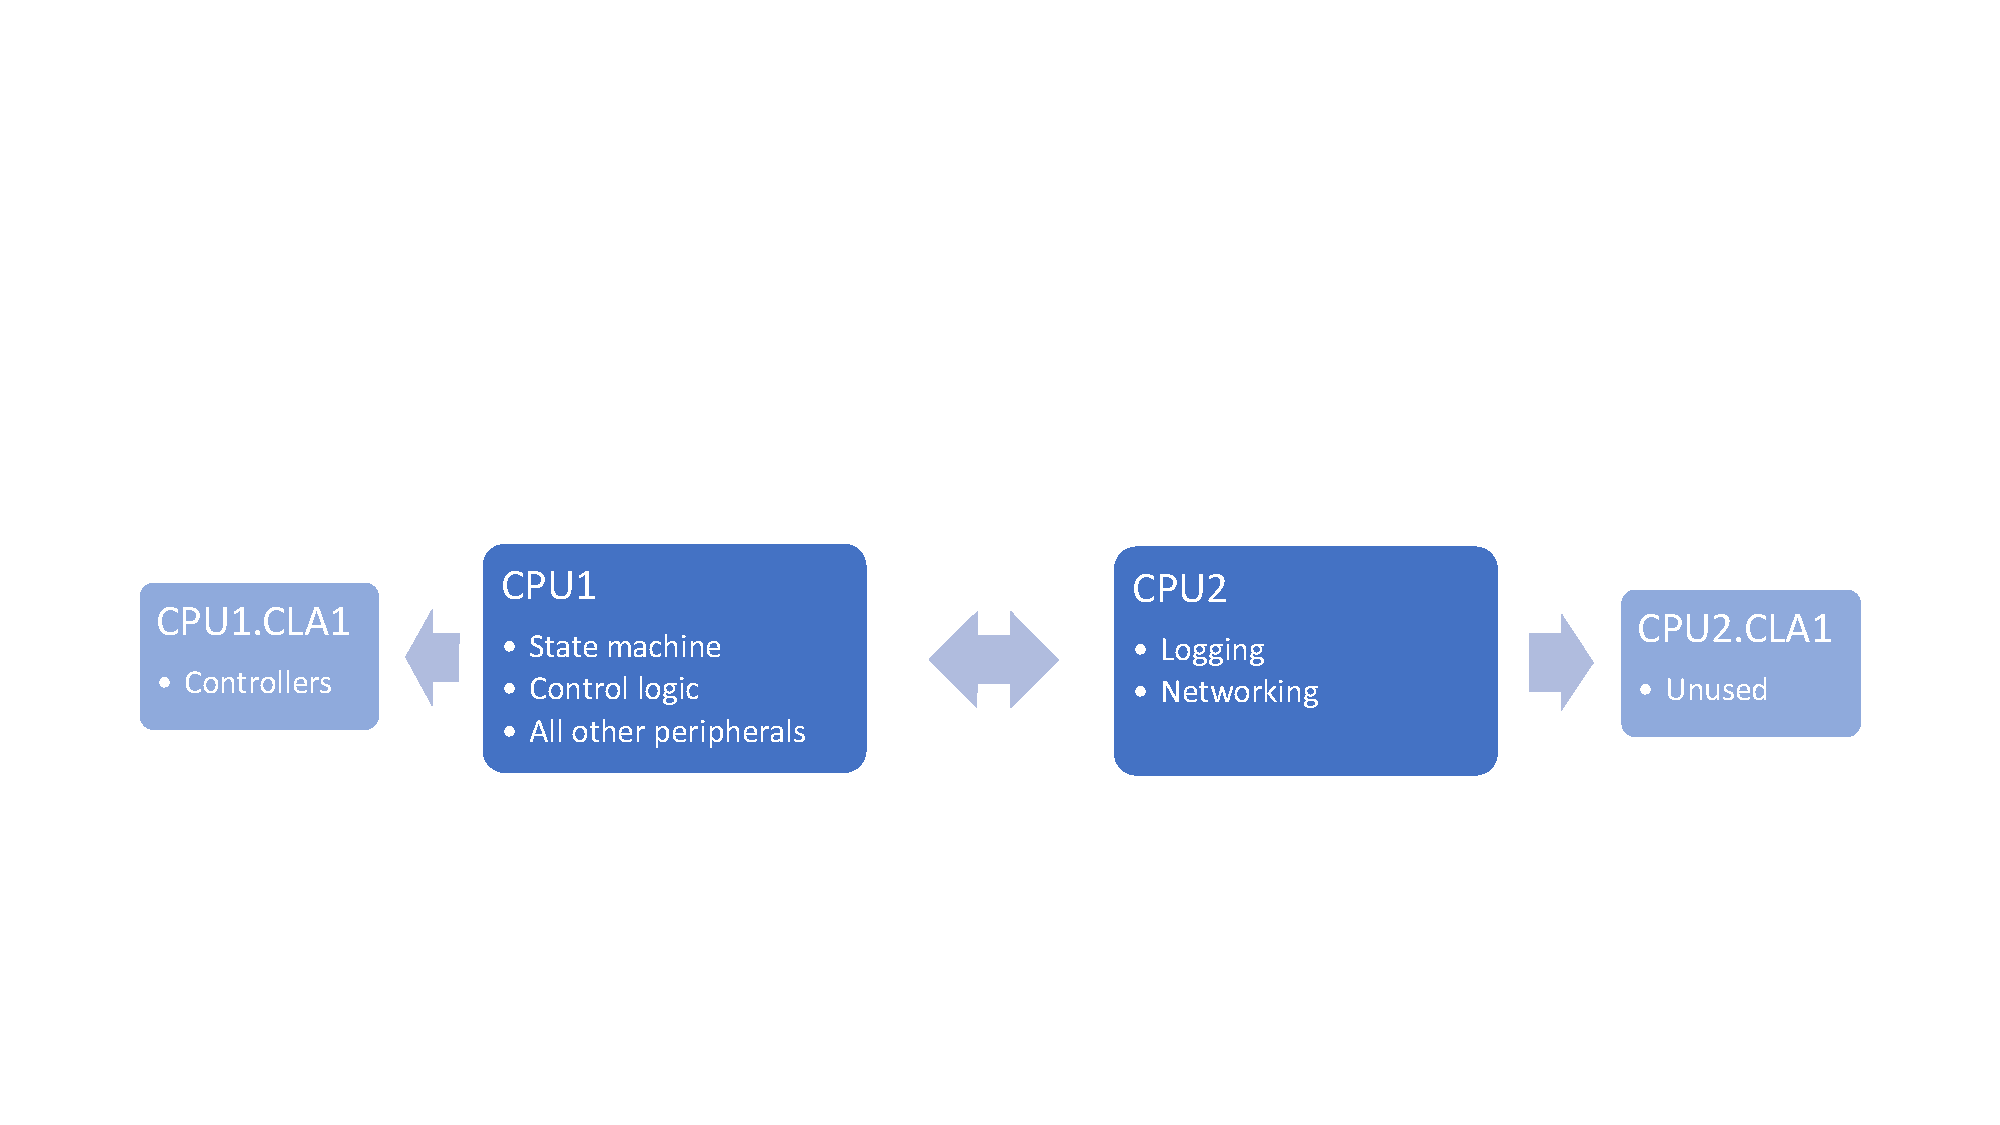
\includegraphics[width=1.0\textwidth]{./figures/system_structure.pdf}
    \caption{Division of tasks between processors and co-processors.}
    \label{fig:system_structure}
\end{figure}

Figure~\ref{fig:system_structure} shows the division of tasks between the two CPU cores and one of the Control Law Accelerator (CLA) co-processors. CPU runs most drivers and handles the control logic and state machine. All sensor data is processed on this core and all control decisions are made on it as well. This consolidates the data processing and control logic in one program without the need for concurrency control that could be subject to hard to find bugs.

CPU2 is dedicated to Logging and Networking. The main constraint for this is that the FAT file system is computationally heavy and, as will be discussed in section~\ref{logging}, is hard to implement asynchronously. In order to reduce the performance impact, logging was separated onto the second core. However, since the Ethernet controller uses the same SPI bus as the SD-card and only one CPU core can be the master of each peripheral (in this case one of the SPI interfaces), networking also needs to be handled on the second core.

Two control algorithms for traction and yaw control must execute regularly in precise intervals and therefore stand in conflict with the asynchronous nature of the remaining system. Furthermore, as they were developed by other people who did not necessarily have detailed knowledge of the system, it made sense to provide an isolated environment for the execution of the controllers.

The CLA co-processor runs at the same frequency as the associated CPU core but executes code independently. It is assigned areas of the associated CPU's dedicated RAM for program and data space. As the CLA co-processor is designed to run controllers, it can be assigned up to eight function pointers, which represent tasks. These tasks can be triggered from peripherals but also from software running on the CPU. Once a task is triggered, it runs to completion. Although the instruction set for the CLA is separate and significantly more limited, these other features make the CLA perfectly suited for the task.

\subsection{Module life-cycle}

All modules and drivers follow a similar structure. This structure mainly consists of three functions that are called at different times during the module life-cycle as illustrates in Figure~\ref{fig:module_lifecycle}: \mintinline{c}{init()}, \mintinline{c}{configure()} and \mintinline{c}{update()}.

\begin{figure}[H]
    \centering 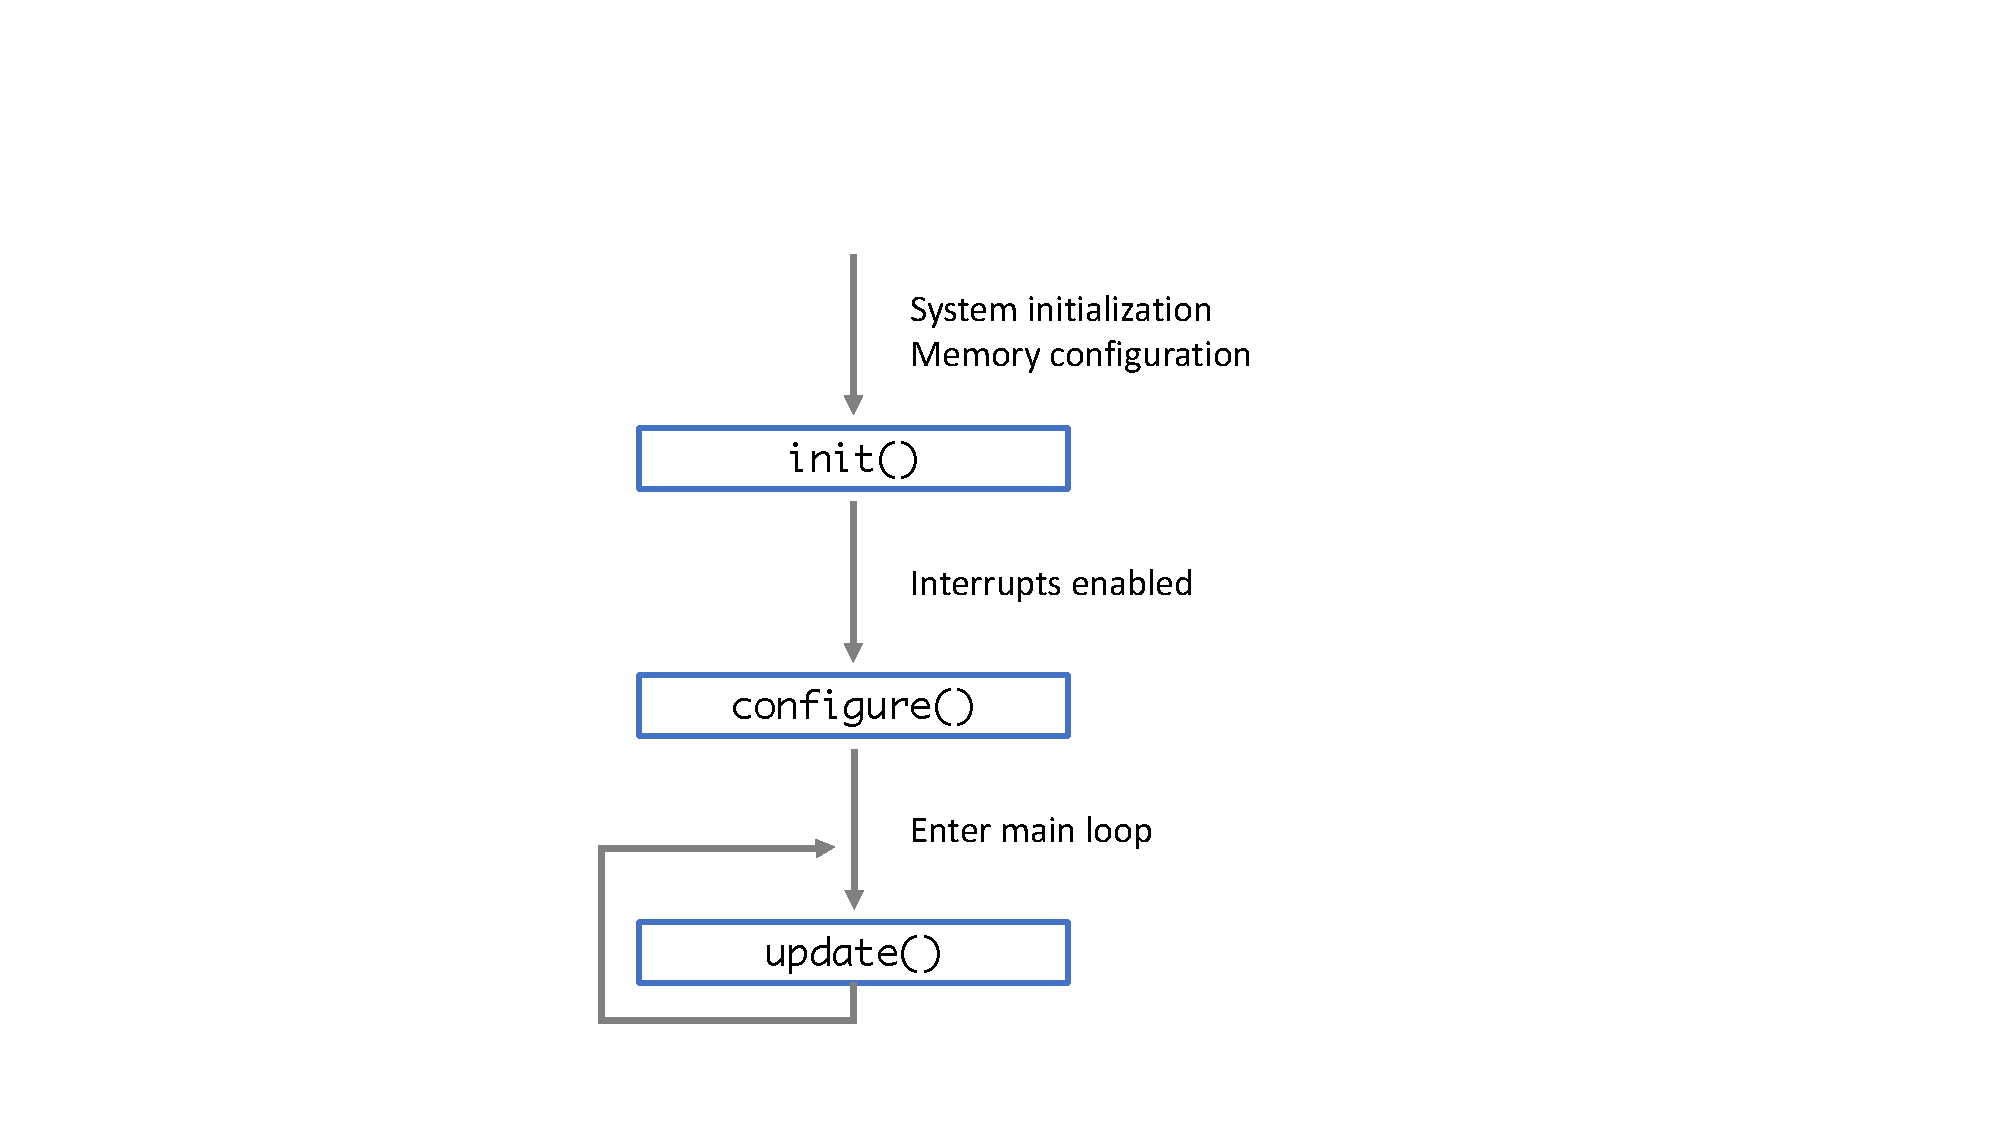
\includegraphics[width=0.5\textwidth]{./figures/module_lifecycle.pdf}
    \caption{Life-cycle of each module in the system.}
    \label{fig:module_lifecycle}
\end{figure}

Immediately after system initialization and memory configuration is complete, \mintinline{c}{init()} is called to allow modules to perform initialisation routines, configure peripherals and enable required interrupts. However, interrupts remain globally disabled for the duration of these function's execution.

Some drivers require further initialisation after interrupts have been enabled. Mostly this involves the configuration of an external device such as the Ethernet Controller, SD-card and laser distance sensors. For these initialisation sequences require fully functional communication and therefore interrupts. This is the purpose of the \mintinline{c}{configure()} functions.

After start-up is complete the processor enters the main loop. At each iteration of the loop the \mintinline{c}{update()} function of each module is called. If the module does not need to perform any computation at that time it immediately returns. Several modules use internal finite state machines in order to allow for asynchronous execution.

\subsection{Data-flow}

\begin{figure}[H]
    \centering 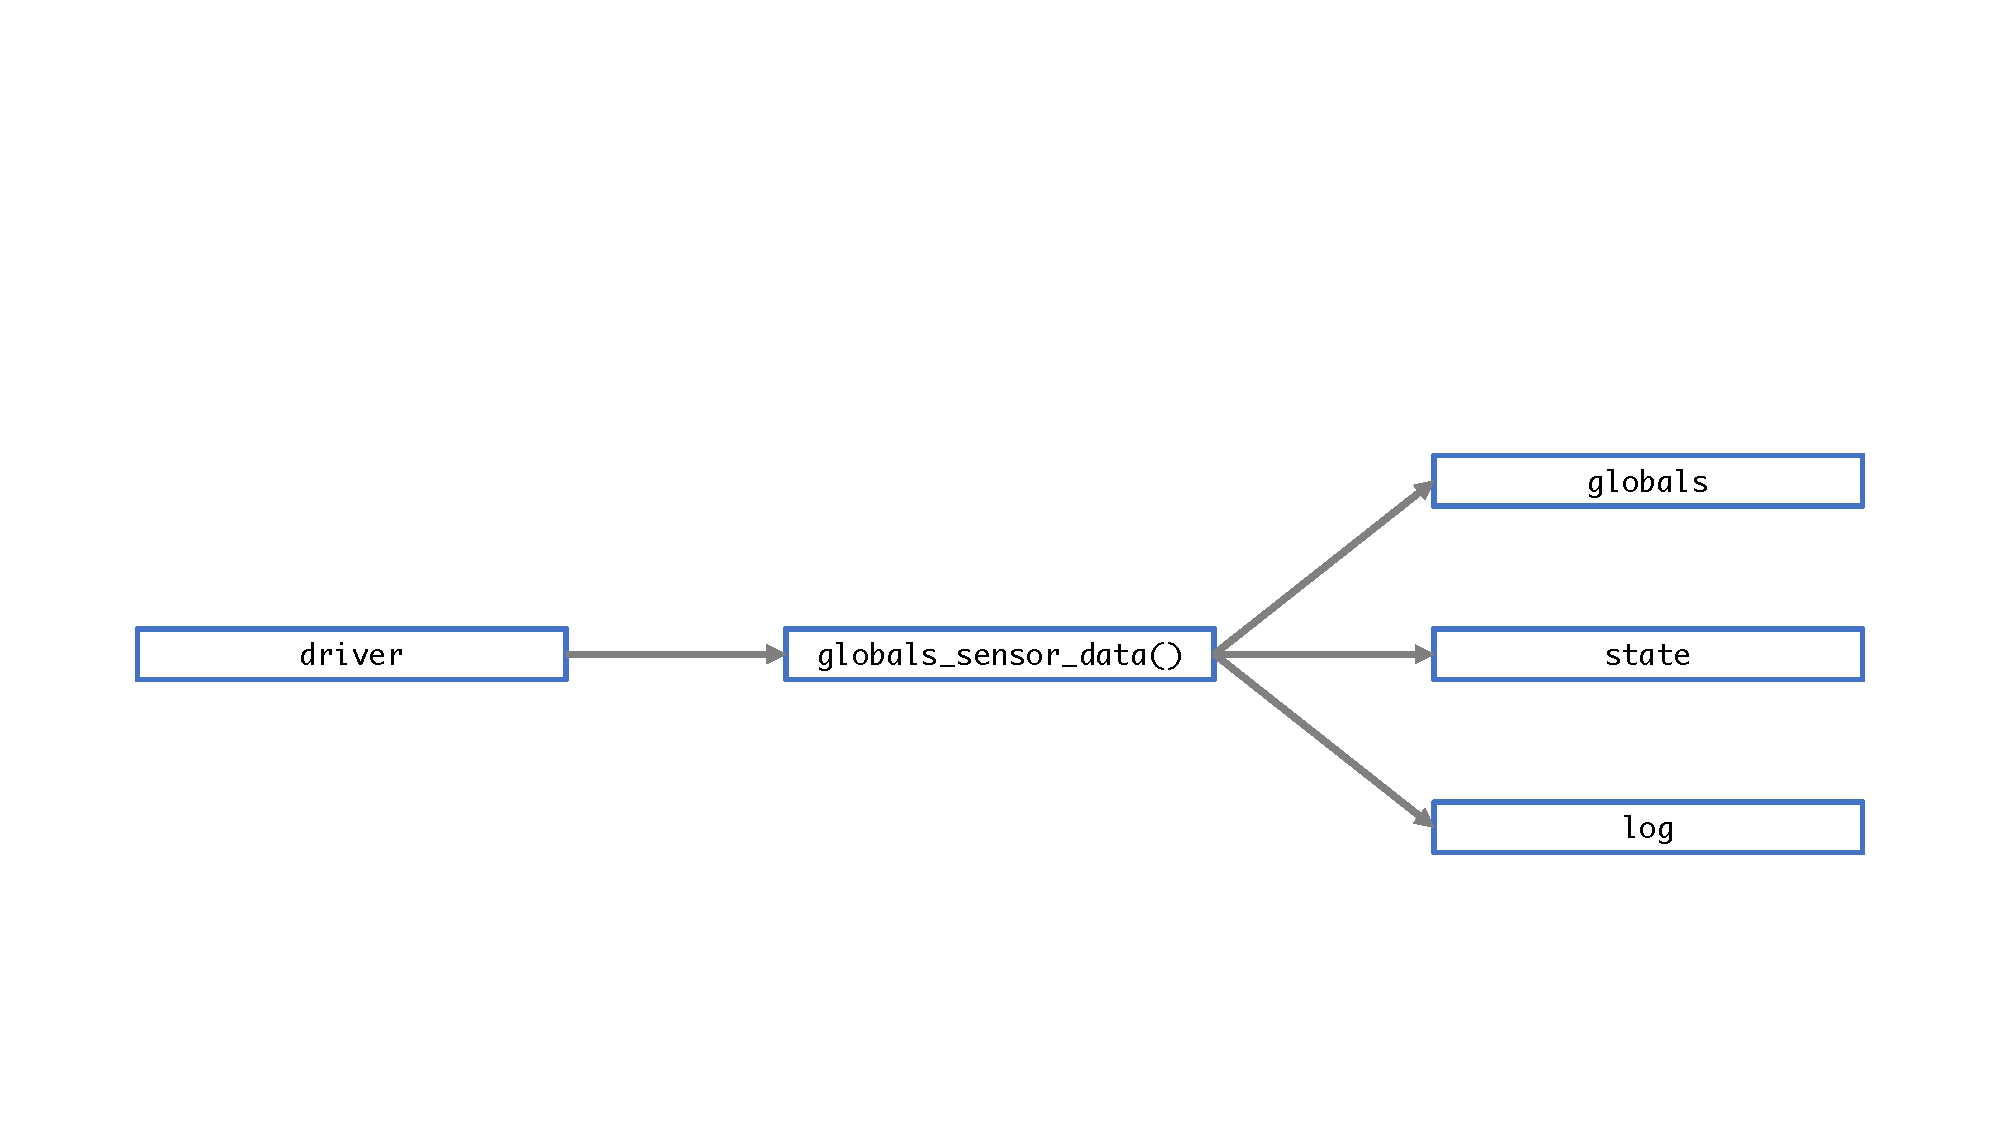
\includegraphics[width=1.0\textwidth]{./figures/dataflow.pdf}
    \caption{Flow of sensor data and derived data.}
    \label{fig:dataflow}
\end{figure}

All data processing is centralised using the \mintinline{c}{globals_sensor_data()} function. The concept is to simplify how data is distributed throughout the program. Drivers call \mintinline{c}{globals_sensor_data()} whenever a new data point is gathered from a sensor. Derived data such as velocity or location is also collected through this function. In this way the data flow is abstracted from the driver layer improving modularisation, maintainability and flexibility.

Once a data point has been collected by a call to \mintinline{c}{globals_sensor_data()}, the data can be stored to a global structure for use by other modules and used to to update the global finite state machine. Additionally, all data points are logged as will be described in Section~\ref{logging}.

\section{Networking}

The network protocol needs to be resistant to packet loss and unstable network connections, while still providing a steady stream of data. Unlike the event-based logging system (Section~\ref{logging}) telemetry data transmitted over the network can be relatively infrequent and there is no data that must be delivered at a higher rate than other data. Therefore I implemented the protocol using UDP packets. The structure listed in Appendix~\ref{telemetry_frame} holds all the data that needs to be transmitted. It fits into a single UDP packet without segmentation. This makes it very efficient to transmit telemetry and resistant to occasional packet loss as only one packet is needed to observe the pod's state.

For controlling the pod remotely from the control panel the protocol follows an analogous scheme using a control frame consisting of the following structure.

\begin{minted}{c}
struct ctrl_frame {
    uint16_t set_state;     // 0: D.C. / ..: the state
    uint16_t aux_power;     // 0: D.C. / 1: OFF / 2: ON
    uint16_t precharge;     // 0: D.C. / 1: OFF / 2: ON
    uint16_t battery;       // 0: D.C. / 1: OFF / 2: ON
    uint16_t brakes;        // 0: D.C. / 1: DISENGAGE / 2: ENGAGE
    uint16_t low_speed;     // 0: D.C. / 1: BACK / 2: STOP / 3: FWD
    uint16_t clear_fault;   // 0: D.C. / 1: CLEAR
    uint16_t reset_run;     // 0: D.C. / 1: RESET
    uint16_t bms_power;     // 0: D.C. / 1: OFF / 2: ON
    uint16_t eject_sd_card; // 0: D.C. / 1: EJECT
};
\end{minted}

Both the telemetry frame and control frame must be sent (and received) regularly in order for the pod and the control panel to check connectivity and enter a safe state should it fail. Therefore the fields in the control frame are usually zero and a non-zero value indicates a control command.

Although the networking drive primarily executes on CPU2, a small portion also executes on CPU1. This is necessary, since all telemetry data originates from CPU1. Rather than placing data in global structures unnecessarily, the telemetry frame is simply assembled on CPU1 and then read by the DMA controller on CPU2. Similarly, CPU2 receives incoming control packets and CPU1 decodes them and executes any control commands. This process is illustrated by Figure~\ref{fig:networking_structure}.

\begin{figure}[H]
    \centering 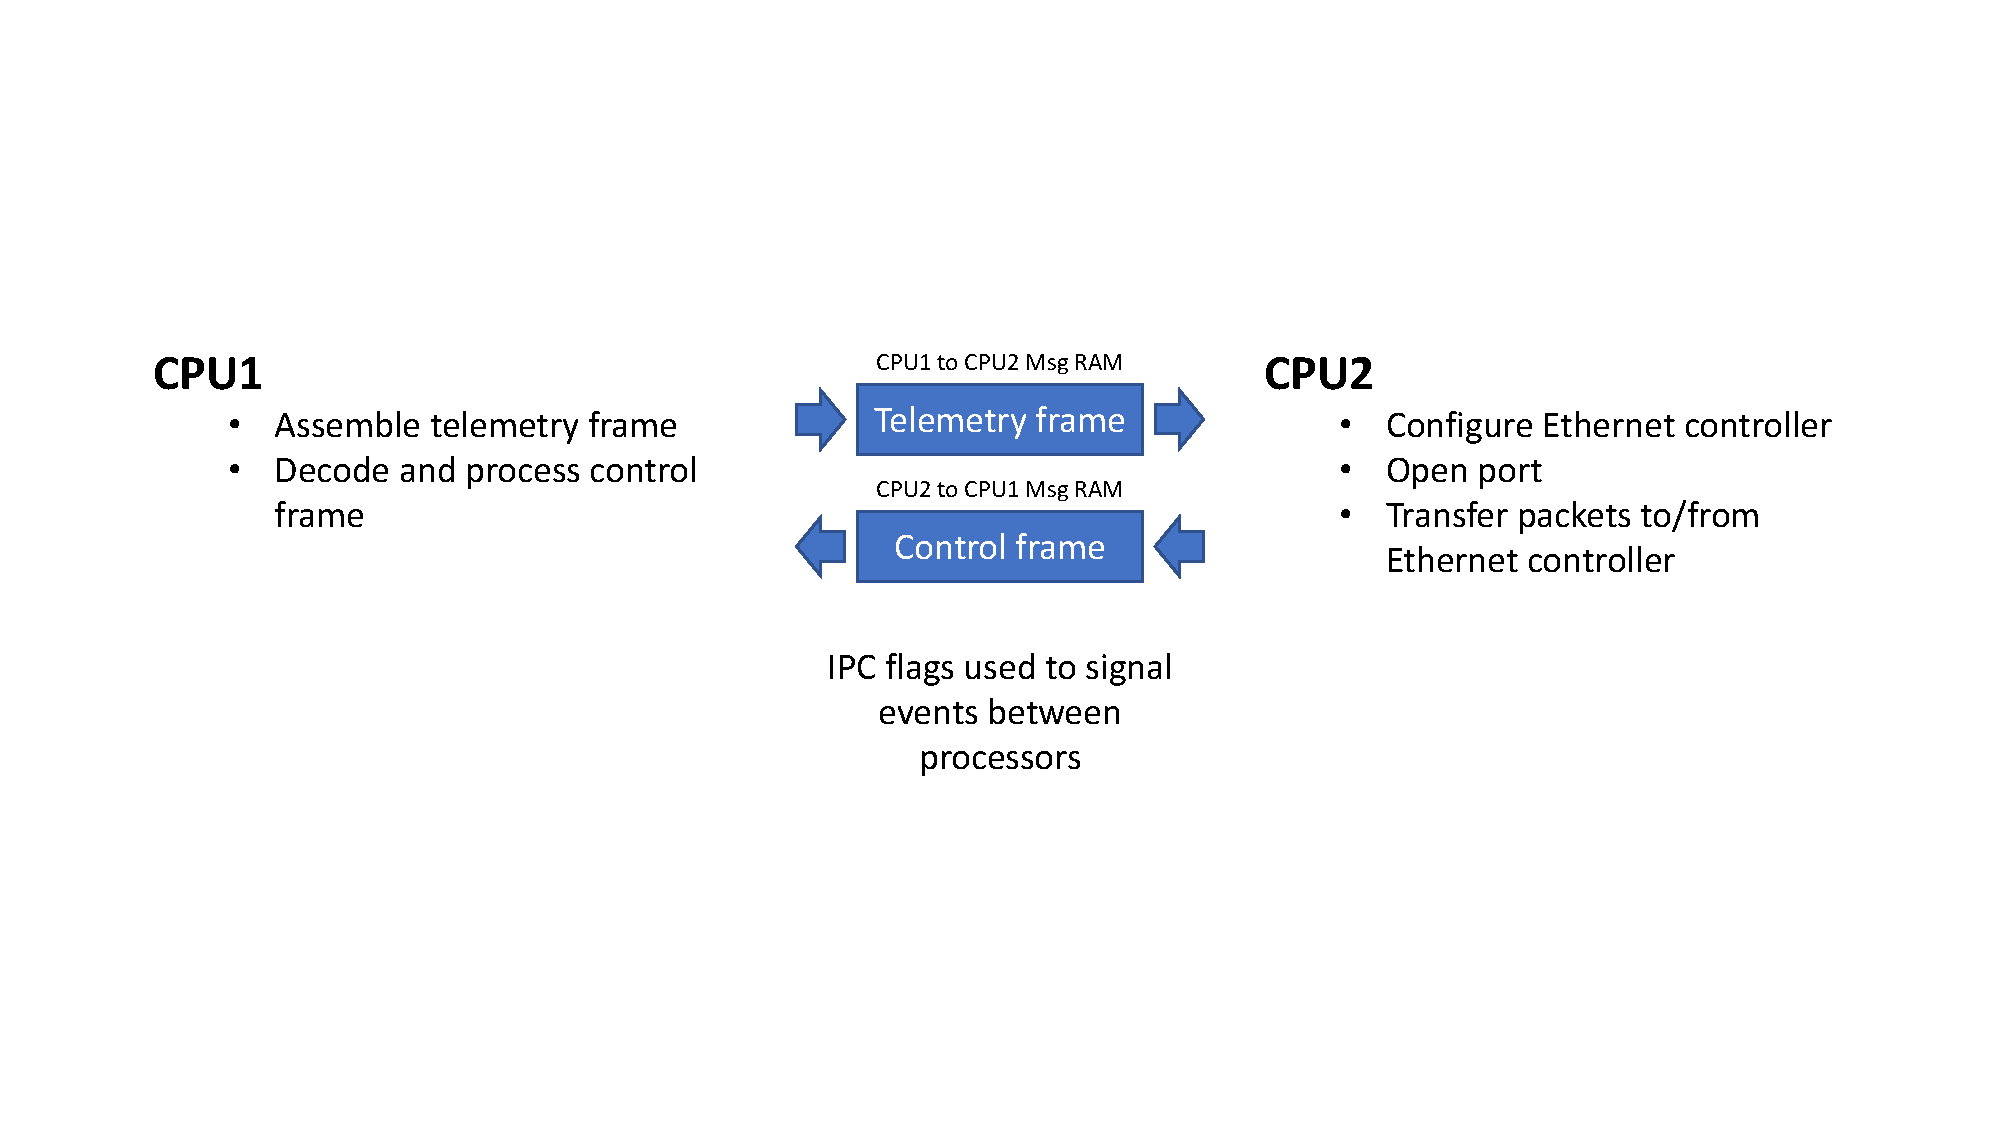
\includegraphics[width=1.0\textwidth]{./figures/networking_structure.pdf}
    \caption{Structure of networking driver.}
    \label{fig:networking_structure}
\end{figure}

The telemetry and control frames are written to Message RAM, which is a shared memory area specifically designed for this kind of usage. It consists of two 1K regions, one writeable only by CPU1 and one only writeable by CPU2. The telemetry frame only consists of 76 16-bit words and therefore easily fits into the Message RAM. The micro-controllers Interprocessor Communication (IPC) module further provides flag registers. The networking driver uses IPC flags to notify the other CPU of the following events:

\begin{itemize}
    \item CPU1 $\rightarrow$ CPU2: Telemetry frame assembled and ready for transmission.
    \item CPU2 $\rightarrow$ CPU1: Telemetry frame has been transmitted and can be overwritten.
    \item CPU2 $\rightarrow$ CPU1: Control frame received.
    \item CPU1 $\rightarrow$ CPU2: Control frame has been processed and can be overwritten.
\end{itemize}

To achieve the highest possible performance all SPI communication with the Ethernet controller is implemented using the micro-controller's DMA controller. Since the SPI interface can be used with a 16-level FIFO extension, the DMA controller can operate in Burst mode. This means that the data is transferred in bursts of 16 words until the transfer has completed. The next bust is triggered by the FIFO interrupt which can be configured to assert at a specific level. For this implementation it is configured to trigger when the FIFO is empty but depending on the size of the bursts this can be optimized.

The following listing shows the process of configuring channel one of the DMA controller for transmission of a buffer at \mintinline{c}{src} of length \mintinline{c}{len}. Notice that the burst length must be a divisor of the total buffer size. This is because the DMA controller cannot handle bursts of different lengths.

\begin{minted}{c}
void spia_tx_dma(uint16_t *src, uint16_t len)
{
    uint16_t burst;

    // Calculate largest burst length
    for (burst = 16; len % burst; burst /= 2) ;

    // Reset the TX FIFO
    SpiaRegs.SPIFFTX.bit.TXFIFO = 0;

    // Configure DMACH1 for SPIA TX
    DMACH1AddrConfig(&SpiaRegs.SPITXBUF, src);
    DMACH1BurstConfig(burst - 1, 1, 0);             // Burst size, src step, dest step
    DMACH1TransferConfig((len / burst) - 1, 1, 0);  // Number of transfers, src step, dest step
    DMACH1ModeConfig(DMA_SPIATX,PERINT_ENABLE,ONESHOT_DISABLE,CONT_DISABLE,
                     SYNC_DISABLE,SYNC_SRC,OVRFLOW_DISABLE,SIXTEEN_BIT,
                     CHINT_END,CHINT_ENABLE);

    // Set the TX FIFO interrupt level
    SpiaRegs.SPIFFTX.bit.TXFFIL = 0;

    // Start the DMA transfer
    _spia_tx_dma_done = 0;
    StartDMACH1();

    // Release the TX FIFO from reset
    SpiaRegs.SPIFFTX.bit.TXFIFO = 1;

}
\end{minted}

The procedure for configuring the DMA controller to read data from the SPI interface is analogous.

Using the DMA controller means that the SPI interface can operate at it's highest possible data-rate without causing significant CPU usage. The clock rate used for the SPI bus is 12,5 MHz.

\section{Logging} \label{logging}

\subsection{File system}

The largest design decision in designing the logging driver was the file system to use. The main requirement was for the logged data to be quickly and easily retrievable. The most commonly used file system on SD-cards is FAT (FAT32 or exFAT). The advantage of the FAT file system in this case is that it can be read with almost any computer making it particularly easy to retrieve log files. On the other hand, FAT is very inefficient unless the FAT table (which on larger storage devices is very large) can be cached in memory. If the FAT table is not cached, it must be read block by block every time a file is being written and a new block is needed. In embedded applications like this one, it is usually not possible to cache the FAT table.

Instead of using FAT I also considered employing specialized logging file systems such as log\_fs \todo{insert reference} and Yaffs \todo{insert reference}. These sequentially write to the storage medium and do not need to access any other data structures while writing the file. Although this leads to higher performance while writing, it also makes finding and extracting log data much more complex. Furthermore, it is not possible to read the data on a regular computer without specialised software. For this reason, I decided to use the FAT file system and write the log data to CSV files.

Log files are created at system start-up and data is continuously appended until the system shuts down or a manual command is given to close the file and ensure data consistency. The CSV file consists of three columns:

\begin{itemize}
    \item \textbf{timestamp}: The time stamp of the data point measured in milliseconds since system start-up.
    \item \textbf{id}: An integer describing the type of data point or event being logged. IDs are defined by the enumeration listed in Appendix~\ref{log_event}
    \item \textbf{value}: The value being logged.
\end{itemize}

The following listing illustrates the structure of a typical log file:

\begin{verbatim}
timestamp;id;value
4778;41;7
4778;39;348
4778;40;3820
4778;42;24
4778;45;5
4778;43;352
4778;44;3781
4778;46;26
4778;5;0
4778;4;0
4879;38;0
4879;37;0
4879;36;0
4879;1;6
4879;2;4
\end{verbatim}

Although beneficial, implementing a specialised FAT driver would not have been possible within the time-frame of this project. Therefore, I decided to use the FatFs\todo{reference} library. At first I attempted to use the newest version of the library. However, the micro-controller uses 16-bit addressable memory and therefore does not support 8-bit data types. Without rewriting large portions of the library it was not possible for it to run without native 8-bit data types. Luckily Texas Instruments includes an older version of the library with ControlSUITE\todo{reference} that is able to run without 8-bit data types.

The FatFs library provides the file system library but an SD-card driver layer also needed to be implemented to provide the interface to the underlying storage medium through the SPI driver. Unlike all other drivers, the SD-card and FAT drivers are not asynchronous. This is mostly due to how the FatFs library operates. Additionally, the data is organized into 8-bit bytes each contained within a 16-bit word which is the smallest possible data type on the processor. Furthermore, due to this constraint the use of DMA is not practical as data mapping is necessary before data can be written to the SPI interface and after it is read from the SPI interface.

Due to the limitations described above, the entire logging driver is fundamentally synchronous and the SD-card driver is implemented using only the FIFO extension of the SPI interface and without DMA. Given more time, a custom FAT driver could be designed specifically for this processor and incorporate the DMA controller and asynchronous operation. Alternatively, a real-time operation system could be used to partially alleviate the problem using threading. Another crude fix to introduce some asynchronism would be to utilize long jumps to context switch out of the logging driver.

\subsection{Event-based logging}

In the logging system implemented in Escher, logging and telemetry data transmission were coupled. The main disadvantage to this was that all data values were logged at the same frequency and no prioritization was possible. Although most sensors on Escher were sampled at the same rate, this is not the case on Mujinga where some sensors such as the laser distance sensors are sampled at around 150Hz and others such as the brake pressure sensors are sampled at 10Hz. Thus, in contrast to Escher, Mujinga's logging system is event-based.

Whenever a new data point is acquired or another system event occurs, a string corresponding to a new line in the CSV log file is generated and appended to a buffer. The following listing shows the procedure for generating the string:

\begin{minted}{c}
// Buffers used to construct string
// ( 8) timestamp (ms)
// ( 1) ;
// ( 5) id
// ( 1) ;
// (20) value
// ( 3) \r\n\0
static char string[38], temp[21];

// Write timestamp
itoa(micros() / 1000, string);

// Write ';'
strcat(string, ";");

// Write id
itoa(id, temp);
strcat(string, temp);

// Write ';'
strcat(string, ";");

// Write value
itoa(value, temp);
strcat(string, temp);

// Write "\r\n"
strcat(string, "\r\n");
\end{minted}

\subsection{Dual-core structure}

Similar to the networking driver, the logging driver is also divided between both cores since all data that needs to be logged is generated on CPU1 while CPU2 maintains the file system and writes to the log file. Figure~\ref{fig:logging_structure} illustrates the cross-core structure.

\begin{figure}[H]
    \centering 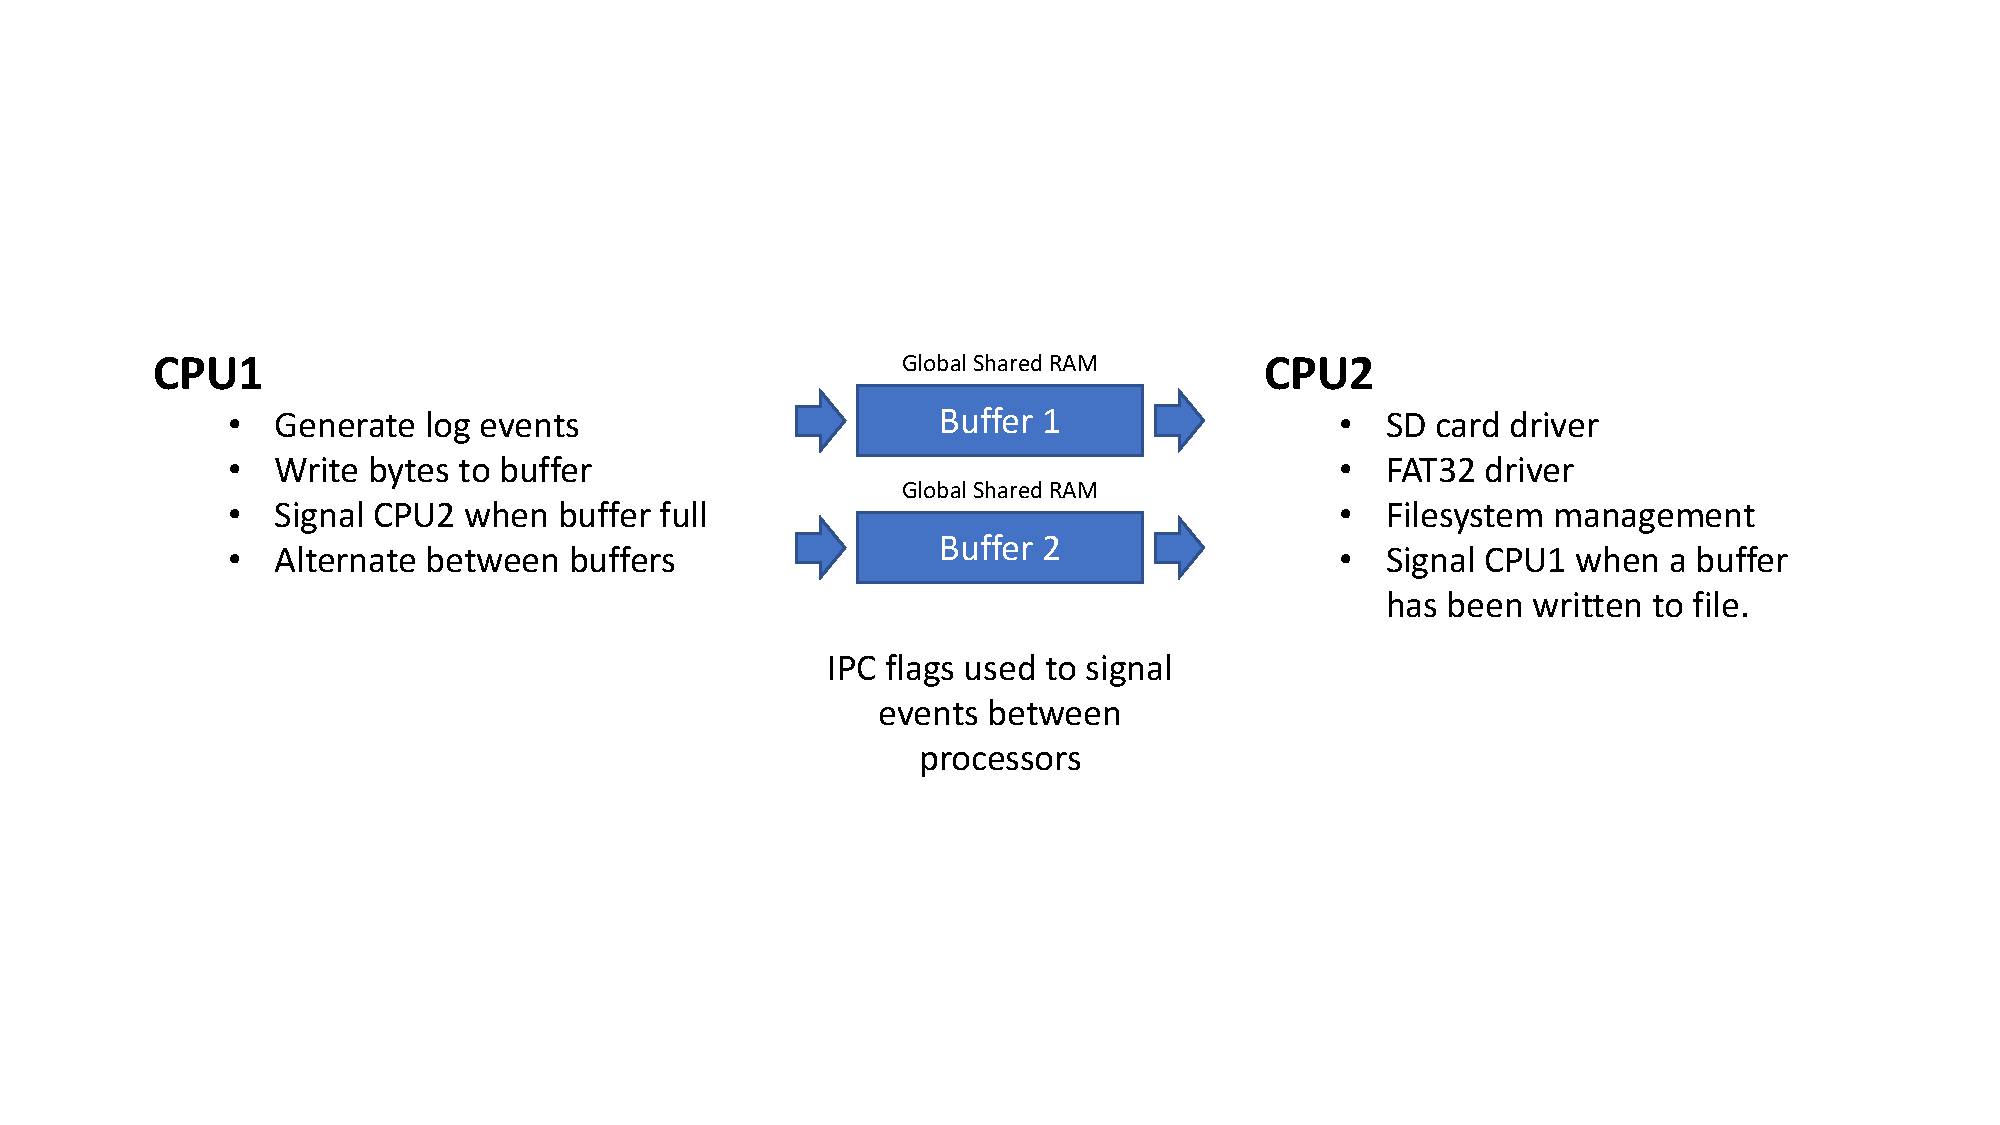
\includegraphics[width=1.0\textwidth]{./figures/logging_structure.pdf}
    \caption{Structure of logging driver.}
    \label{fig:logging_structure}
\end{figure}

Two buffers in shared memory (writeable by CPU1) are used to hold the next segments of the log file as they are generated. Once a buffer is full an IPC flag is used to communicate this to CPU2 and CPU1 continues to write to the other buffer. CPU2 writes the buffer out to the SD-card. Once this is complete it uses an IPC flag to signal to CPU1 that the buffer can be overwritten again and the process repeats.

Usually this kind of functionality would be achieved using a ring-buffer. However, in this particular situation this approach does not work as well for two reasons:

Firstly, for performance reasons relating to the SD-card, performance is best when the file is written in consecutive blocks of 512 byte. Additionally, this reduces the overhead produced by reading the FAT table since every block will only be accessed to once.

Secondly, to optimized the performance of the FatFs library by reducing overheads, the write operation should be invoked infrequently with large chunks of data rather than frequently with smaller chunks of data. When using a ring-buffer a chunk of data may not be consecutively stored in memory leading to at least two invocations of the write operation rather than one.

Given these constraints, an optimally implemented and configured ring-buffer would operate identically to the separate buffers approach explained above. Each buffer consists of 4kB. The trade-off leading to this size is explained in Section~\ref{logging_perf}.

\section{External Analog-To-Digital Converter (ADC)}

Some of the code for communicating with the external analog-to-digital converter was based on the software from Escher, since the same component was used. However, the code has been optimized to reduce communication to 32 SPI clock cycles per measurement.

At start-up the external ADC is reset to make sure it is in a known state. After initialising the ADC, it is configured to use it's internal 2.5V reference and deliver 100 Samples per second. The ADC reads data form 10 channels so this sample rate provides a constant sampling rate of 10Hz. Single-shot conversion mode is used so that the ADC provides a single conversion before the channel can be changed for the next conversion.

In the main loop the processor waits for the $\overline{DRDY}$ signal from the ADC to go low indication that the last conversion has completed. Next, the data sequence illustrated by Figure~\ref{fig:adc_spi} delivers the 24-bit value of the conversion and starts the next conversion.

\begin{figure}[H]
    \centering \includegraphics[width=1.0\textwidth]{./figures/"ADC SPI1".PNG}
    \caption{Data flow on the SPI bus with the external ADC.}
    \label{fig:adc_spi}
\end{figure}

The following commands and data can be observed in Figure~\ref{fig:adc_spi}:

\begin{itemize}
    \item MCU $\rightarrow$ ADC: (MOSI)
    \begin{itemize}
        \item \textbf{42 00}: Write one byte to input multiplexer register.
        \item \textbf{19}: New value for input multiplexer register, selecting next channel.
        \item \textbf{08}: Start conversion command.
    \end{itemize}
    \item ADC $\rightarrow$ MCU: (SOMI)
    \begin{itemize}
        \item \textbf{00}: Status byte.
        \item \textbf{11 A3 5C}: Value of previous conversion.
    \end{itemize}
\end{itemize}

\section{RS485 Bus}

\begin{figure}[H]
    \centering 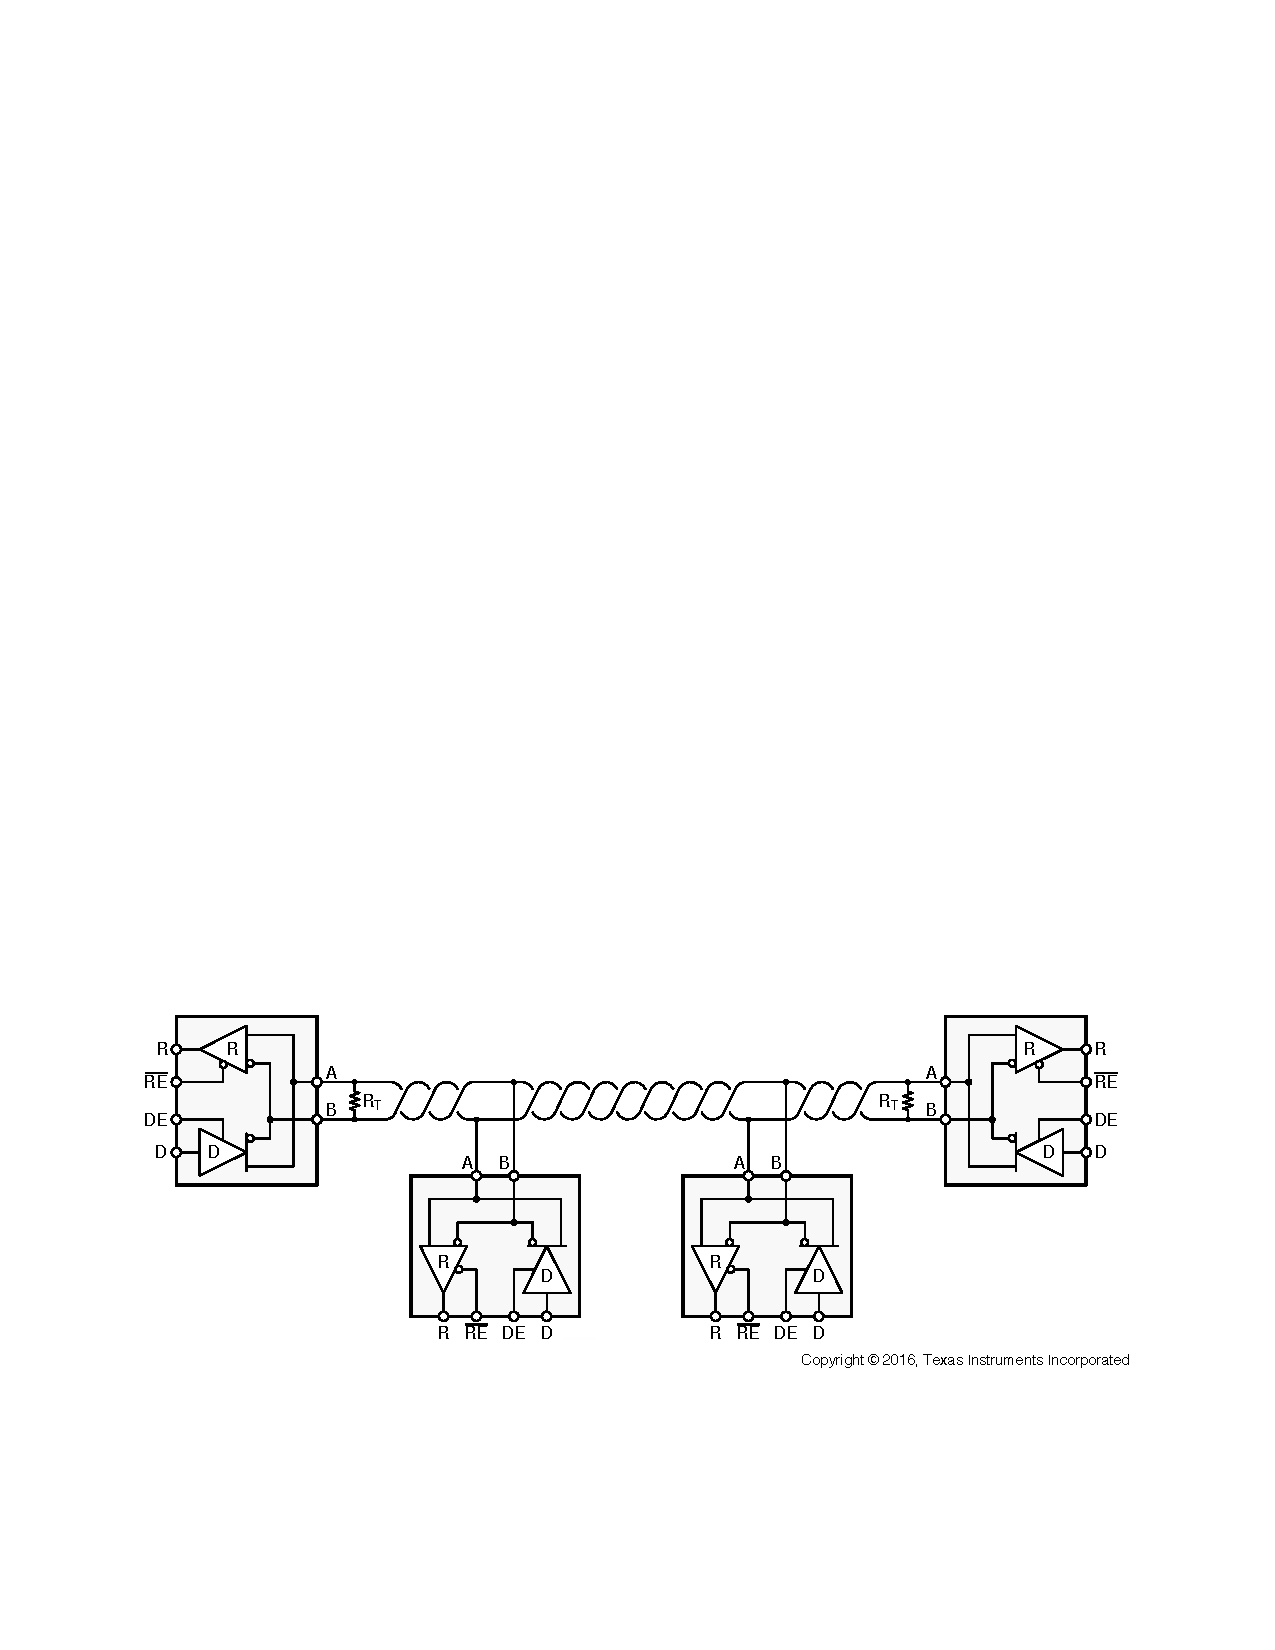
\includegraphics[width=1.0\textwidth]{./figures/rs485_structure.pdf}
    \caption{Structure of RS485 bus - Texas Instruments SN65HVD7x Datasheet\cite{RS485TransceiverDatasheet}}
    \label{fig:rs485_structure}
\end{figure}

As mentioned before, the data format used in the RS485 bus standard is identical to standard serial (RS232) and therefore supported by the Serial Communication Interface (SCI) built into the micro-controller. However, RS485 uses differential signalling. Therefore, a transceiver is required. Additionally, the bus structure means that only a single device may transmit at a time. For the micro-controller this has more complicated implications. The transceiver can only receive data if it is not transmitting, meaning that the micro-controller must signal produce an RTS signal ($\overline{RE}$ and $DE$) to determine which state the transceiver is in.

Using the 16-level FIFO extension of the SCI interface, the drivers are able to operate asynchronously by pushing up to 16 words into the FIFO and continue processing while these are transmitted. The need to control the RTS signal would now break this asynchronism since it must be asserted immediately before beginning the transmission and immediately after the transmission completes to allow other devices to use the bus. Next, I will describe a solution which allows for asynchronism again using interrupts.

First, the FIFO interrupt is configured to trigger once the FIFO is empty. However, the interrupt triggers when the last word in the FIFO has been transferred to the transmit buffer. There is no interrupt that can trigger when the last word has been fully transmitted. Therefore, the interrupt service routine triggers a CPU timer which triggers another interrupt after the duration it takes to transmit the final word. This time can be calculated using the BAUD rate. The interrupt service routine for the timer interrupt the de-asserts the RTS signal.

\subsection{OADM}

The RS485 protocol used by the Baumer OADM\todo{reference} laser distance sensors is simple. Each sensor has a unique ID (a single-digit non-zero number), which is configured during installation. The micro-controller requests the current sensor reading from a specific sensor using it's ID and the sensor responds with the reading. The request consists of four characters where \texttt{*} represents the ID of the desired sensor: \texttt{\{*M\}}. An example reply from the sensor looks as follows: \texttt{\{*MM0448564\}}.

The following listing shows the \mintinline{c}{update()} function for the OADM driver module. A simple state machine with two states allows the the module to be reset to the \mintinline{c}{READY} state, which is also it's initial state.

\begin{minted}{c}
void oadm_update()
{

    uint16_t BUF[12];
    uint32_t reading;
    static uint64_t time_requested = 0;

    switch (state) {

    case READING:
        // Check if we have received the full reply from the sensor
        if (micros() - time_requested > 100000ull) {
            state = READY;
            return;
        } else if (scic_available() < 12) {
            return;
        }

        // Read the sensor's reply
        scic_rx(BUF, 12);

        // Parse the response
        BUF[9] = '\0';
        reading = map(atoi((char *) BUF + 4), 0, 8191, 0, 120000);  // um

        // Emit the reading
        globals_sensor_data(current_sensor == 1 ? SENSOR_DIST_RAIL_TOP_FRONT : SENSOR_DIST_RAIL_TOP_BACK, &reading);

        // Read from the next sensor
        current_sensor = (current_sensor % NUM_SENSORS) + 1;

        // Fall through to READY case
        /* no break */

    case READY:
        // Prepare the request
        BUF[0] = '{';
        BUF[1] = '0' + current_sensor;
        BUF[2] = 'M';
        BUF[3] = '}';

        // Send the request
        scic_tx(BUF, 4);

        // Keep track of time
        time_requested = micros();

        // Go to READING state
        state = READING;

        break;

    }

}
\end{minted}

\subsection{OM70}

The Baumer OM70\todo{reference} sensors use different RS485 bus settings and also employ a more complex protocol. Nonetheless, the principal of operation is the same except that the sensors must be put into an RS485 enabled mode using an RS485 lock command at start-up. However, a problem arises from the reply from the sensor being significantly longer. The following few lines are example responses from the sensor.

\begin{verbatim}
:01A;108.648;0;2DBB\r\n
:01A;108.577;13;921D\r\n
:01A;NaN;12;B54E\r\n
\end{verbatim}

The replies from this sensor are up to 22 characters long. That is more than the 16 characters that fit into the FIFO of the SCI. This is an issue as without using the FIFO the driver cannot operate asynchronously. Using DMA would alleviate this problem but unfortunately the DMA controller on this micro-controller cannot access the SCI. Furthermore, the length of the reply from the sensor is variable and so the DMA controller would not be well suited to the task.

To prevent a FIFO overflow, an interrupt on the receiving FIFO is configured to trigger when the first 13 characters of a reply have been received. The interrupt service routine then reads the first segment of the reply. The second segment can then be read later without the FIFO overflowing.

\section{CAN Bus}

The CAN bus is designed to be deployed in automotive applications. Mujinga incorporates multiple devices that use the CAN bus. The micro-controller conveniently incorporates a CAN interface and the Launchpad includes a CAN transceiver, so no additional hardware was necessary to support the CAN bus. The built-in CAN interface uses a dedicated Message RAM to store message objects that can be configured to accept CAN messages with an optional CAN ID filter or to hold messages that should be transmitted on the CAN bus. The CAN interface on the micro-controller handles bus arbitration and automatic retransmission so the application only needs to configure message objects with the required properties. To further simplify development using the CAN interface I used a driver library provided by Texas Instruments as part of ControlSUITE\todo{reference}.

\subsection{Inverters}

The motor-controllers (inverters) only use two CAN IDs each: one to receive and one to transmit CAN messages. The details of what message is being transmitted is contained within the message. This is somewhat in contradiction to the original CAN specification where the CAN ID should identify the type of message as it is used as the priority during bus arbitration.

The driver for the inverters configures two message objects for each inverter configured to accept only the corresponding message IDs. The driver then uses the new data register of the CAN interface to check if a new message has been received in the receiving message objects. To send a message to the inverters, it is simply written into the appropriate transmitting message object and configured to be retransmitted until the inverter acknowledges the message.

To kick-start communication, the control panel sends a "Clear inverter faults" command. This leads to the driver transmitting a sequence of messages to each inverter. The messages complete two tasks: First, clear any faults generated by previous error conditions. Secondly, configure the inverter to regularly send the telemetry listed in Section~\ref{spec_inverter}. Most measurements are transmitted every 10 milliseconds.

\subsection{Battery Management Systems (BMS)}

Unlike the inverters the Battery Management Systems adhere to the CANopen\todo{reference?} standard. The BMSs are more passive than the inverters and do not require configuration. They simply start transmit telemetry data at start-up. CANopen messages can be identified by their CAN ID but still contain additional information in the message.

The driver for the BMSs configures one message object for each BMS and for each message that needs to be received configured to only accept the appropriate message ID. Similarly to the inverter driver it uses the new data register of the CAN interface to read message objects whenever new data has been received. The frequency and types of data is hard-coded into the BMS firmware and cannot be configured without intervention from the manufacturer.

\section{Navigation algorithm}

The task of the navigation algorithm is to ensure that the control system can determine the location of the pod and it's velocity.

The primary navigational sensors are optical contrast sensors that recognize optical markings placed in 30m intervals along the track. Although the inverters provide rotational speed measurements from the motors (and therefore the wheels), this on it's own would not be a sufficiently. It is not unlikely, that despite the traction controllers influence the wheels could slip during acceleration. In the event of slipping on the wheels the data from the motors becomes useless for navigational purposes. Furthermore, from a safety point of view, it is not necessary to continuously update the pods position or velocity. The control system only needs to know when the pod has exceeded a pre-defined distance in order to engage the brakes at the correct time. Nonetheless, the rotational speed measurements do take some influence on the navigation algorithm.

Due to the importance of correct navigation and because only one type of sensor is used as a primary input, the system must incorporate fault detection and recovery. The pod has two laser contrast sensors: one at the front and one at the back. This means that at most one laser sensor may miss an optical marking and in almost all situations the system will be able to detect this fault and recover. This is implemented by observing the order in which the sensors trigger. The sensors provide digital output signals that go high when an optical marking is detected, which triggers an interrupt. The following listing shows the interrupt service routine for the front sensor:

\begin{minted}{c}
__interrupt void tape_detection_front_isr(void)
{

    uint64_t now = micros();
    uint64_t min_time_interval = nav_tape_min_time_interval();

    if (now > tape_detection_time_front + min_time_interval) {

        last_tape_detection_time = tape_detection_time_front;
        tape_detection_time_front = now;
        tape_count_front++;

        // Check if the last tape was missed at the back
        if (tape_count_front > tape_count_back + 1) {
            tape_count_back++;
            tape_miss_count++;
        }

        tape_detected = 1;

    }

    EALLOW;
    PieCtrlRegs.PIEACK.all |= PIEACK_GROUP1;    // ACK the interrupt
    EDIS;

}
\end{minted}

The interrupt service routine for the back sensor is analogous. By checking if the number of optical markings detected at the front (\mintinline{c}{tape_count_front}) is at least two greater than at the back (\mintinline{c}{tape_count_back}), the system can determine if the back sensor missed the previous optical marking.

Should the optical marking be dirty it is possible that the sensor triggers twice or more. To prevent the algorithm from registering this as several markings, it checks if a minimum amount of time has passed since the last trigger. This time period is calculated using a call to \mintinline{c}{nav_tape_min_time_interval()} where the average of all rotational speed measurements is used to estimate the amount of time the tape sensor is over an optical marking in order to accurately reject false triggers until the optical marking has been passed. The following listing shows this process:

\begin{minted}{c}
uint64_t nav_tape_min_time_interval()
{

    // Get average of wheel speeds
    int32_t speed = -globals.inverter_fl_speed;
    speed += globals.inverter_fr_speed;
    speed += -globals.inverter_bl_speed;
    speed += globals.inverter_br_speed;
    speed /= 4;

    // Convert speed from rpm to mm/s
    speed *= CONFIG_NAV_WHEEL_CIRCUMFERENCE;
    speed /= 60;

    // Enforce minimum speed
    if (speed < 1000) {
        speed = 1000;
    }

    // Calculate the time interval (us) between the two tape sensors
    uint64_t time = 1000000ull * CONFIG_NAV_TAPE_WIDTH;
    time /= speed;

    // Add a safety margin
    return 8 * time;

}
\end{minted}

To protection against noise, is the input qualification built into the micro-controller that is configured to make sure the signal is stable for 15,3 microseconds before it can lead to an interrupt.

Once the time of detection of an optical marking has been recorded, the location and velocity of the pod can easily be calculated and used to make control decisions and modify the global state.

\section{State Diagram}

As a requirement for the competition, the global control algorithm must be implemented as a finite state machine (FSM). The state diagram is checked and tested during the competition. Therefore, the FSM is designed with simplicity in mind and with the least number of automatic transitions in order to reduce the amount of tests necessary to demonstrate correctness.

\begin{figure}[H]
    \centering 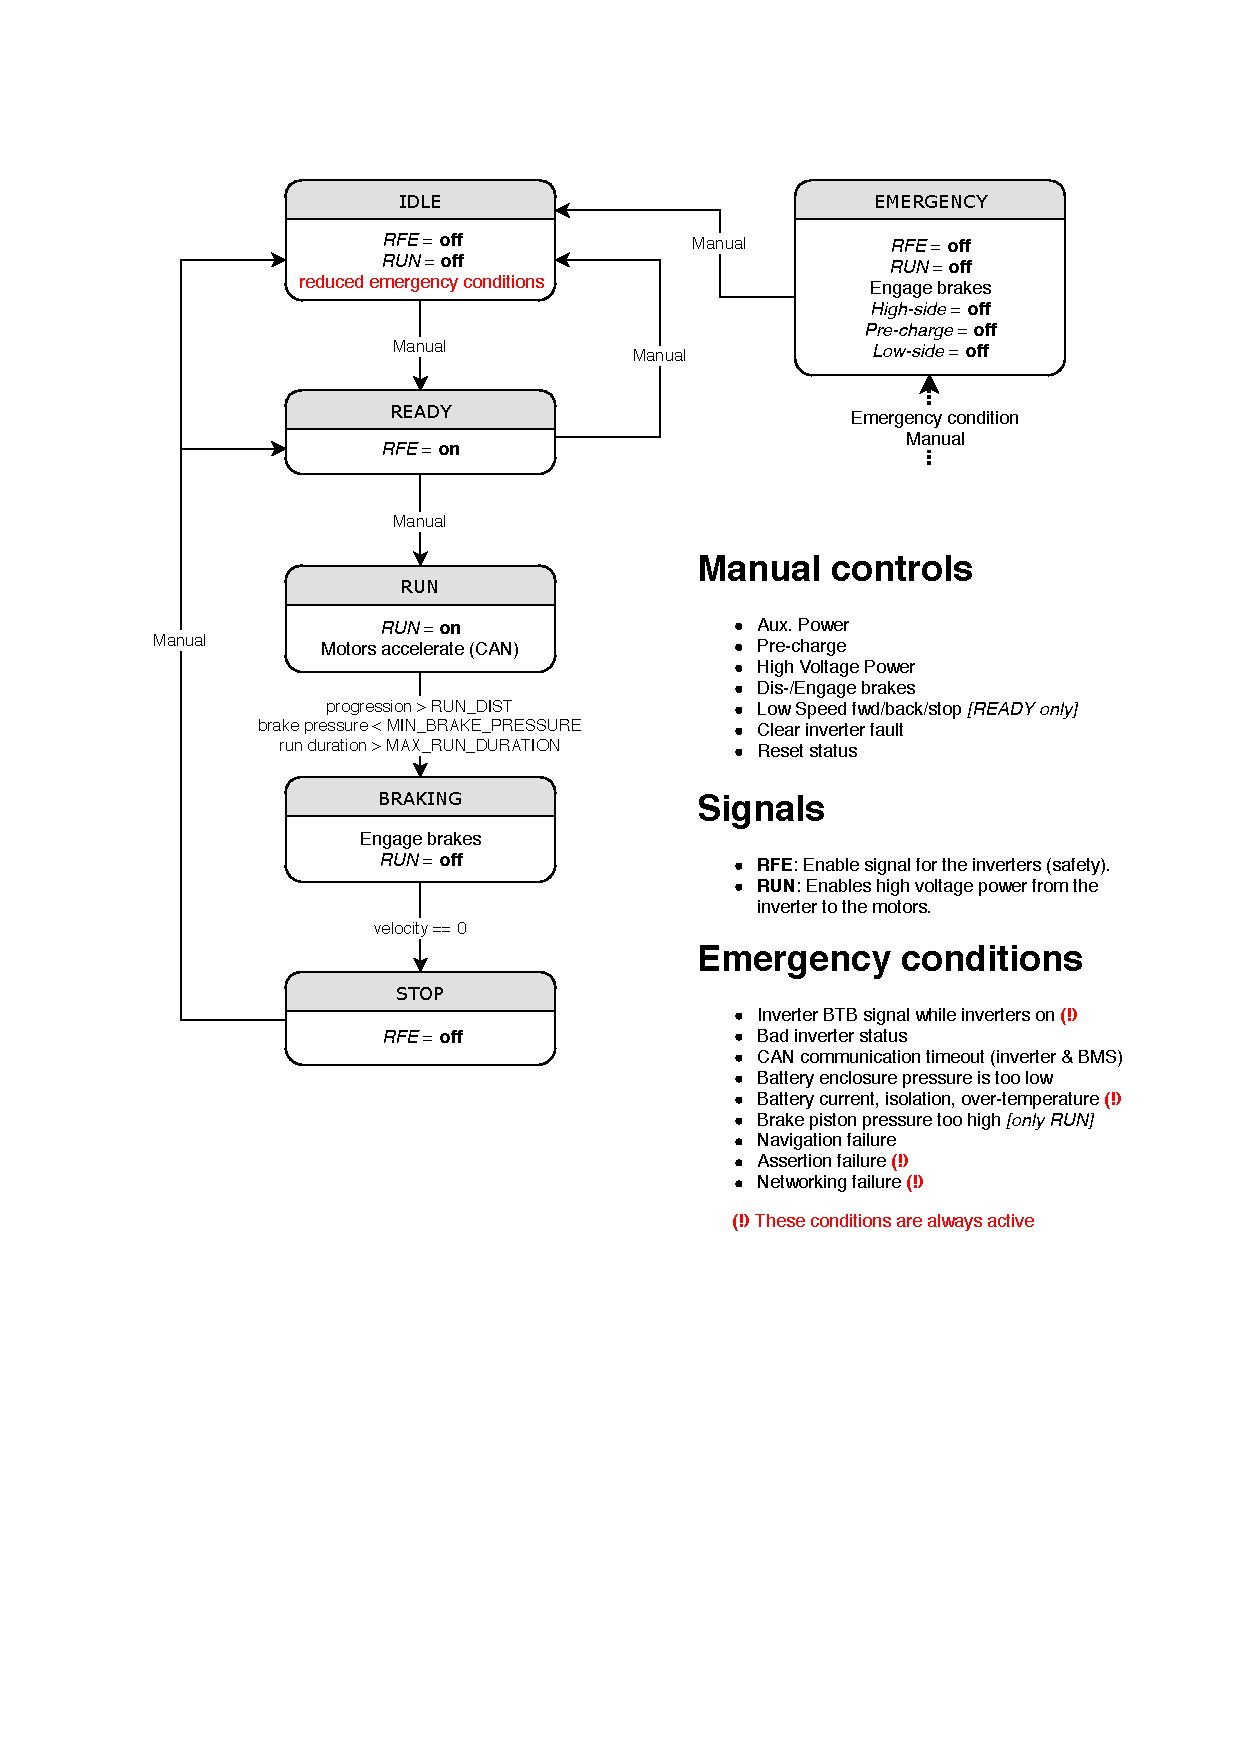
\includegraphics[width=1.0\textwidth]{./figures/state_diagram.pdf}
    \caption{State diagram of the global finite state machine.}
    \label{fig:state_diagram}
\end{figure}

Figure~\ref{fig:state_diagram} shows all states and state transitions. Any state transitions that are not listed in Figure~\ref{fig:state_diagram} are illegal and cannot be executed. The \texttt{EMERGENCY} state can be entered from any other state automatically if an emergency condition occurs or by a manual command form the control panel. All state transitions labelled "Manual" are also executed using a command from the control panel. Additional safety conditions that may prevent manual state transitions apply in some cases.

The \texttt{IDLE} state is intended as the default state when the pod is powered on and stationary. Some emergency conditions are not active in this state as the causes may be cleared by manual intervention with the pod, such as pumping up the brake system to nominal pressure levels.

A nominal run of the pod would consist of the following sequence of states: \texttt{READY} $\rightarrow$ \texttt{RUN} $\rightarrow$ \texttt{BRAKING} $\rightarrow$ \texttt{STOP}. In order to begin a run, the system must transition into the \texttt{READY} state, insuring that the all emergency conditions are negative and the pod is healthy before proceeding. The \texttt{RUN} state represents the acceleration phase of a run and is exited when the pod reaches a pre-defined location, brake failure on at least on of the braking systems appears to be imminent or a pre-defined maximum duration has been exceeded. Once transitioned to the \texttt{BRAKING} state, the motors are disabled by turning off the RUN signal and the brakes are engages. Once the pod has reached a full stop, the pod transitions into the \texttt{STOP} state.

Although the FSM covers all safety critical actions, several other controls are left as manual controls to the user in favour of a simpler FSM. However, in several cases automatic safety checks are still in place that prevent manual actions that would lead to unsafe circumstances.

\section{Control Law Accelerator (CLA)}

As mentioned in Section~\ref{impelementation_structure}, two controllers regulating traction and yaw need to be executed in regular intervals. In order to provide an isolated environment and improve performance, these controllers execute on the CLA. The CLA is a co-processor with a separate instruction set that executes in parallel to the CPU at the same frequency. The CLA is configured with up to eight task vectors (function pointers). A task can then be triggered by a peripheral or by software on the CPU. Once triggered, the task runs until it reaches an \texttt{MSTOP} instruction.

Blocks of the CPU's dedicated RAM can be configured as program and data space for the CLA. Texas Instruments provides a C compiler for CLA instruction set. However, the C compiler only supports a subset of C. The main difference being, that the output programs do not use a stack. Instead a scratch-pad concept is used. As a result recursion is not supported. Even so, the compiler is sufficiently capable for control applications.

In order to pass input arguments to the CLA and return outputs to the CPU, the CLA and CPU share a Message RAM consisting of two 128 word segments. One is writeable only by the CPU, the other is only writeable by the CLA. Variables can be allocated in these segments using a \mintinline{c}{#pragma DATA_SECTION()} directive and then linked in the CPU and CLA code at compile time. Figure~\ref{fig:CLA_communication} illustrates this structure.

\begin{figure}[H]
    \centering 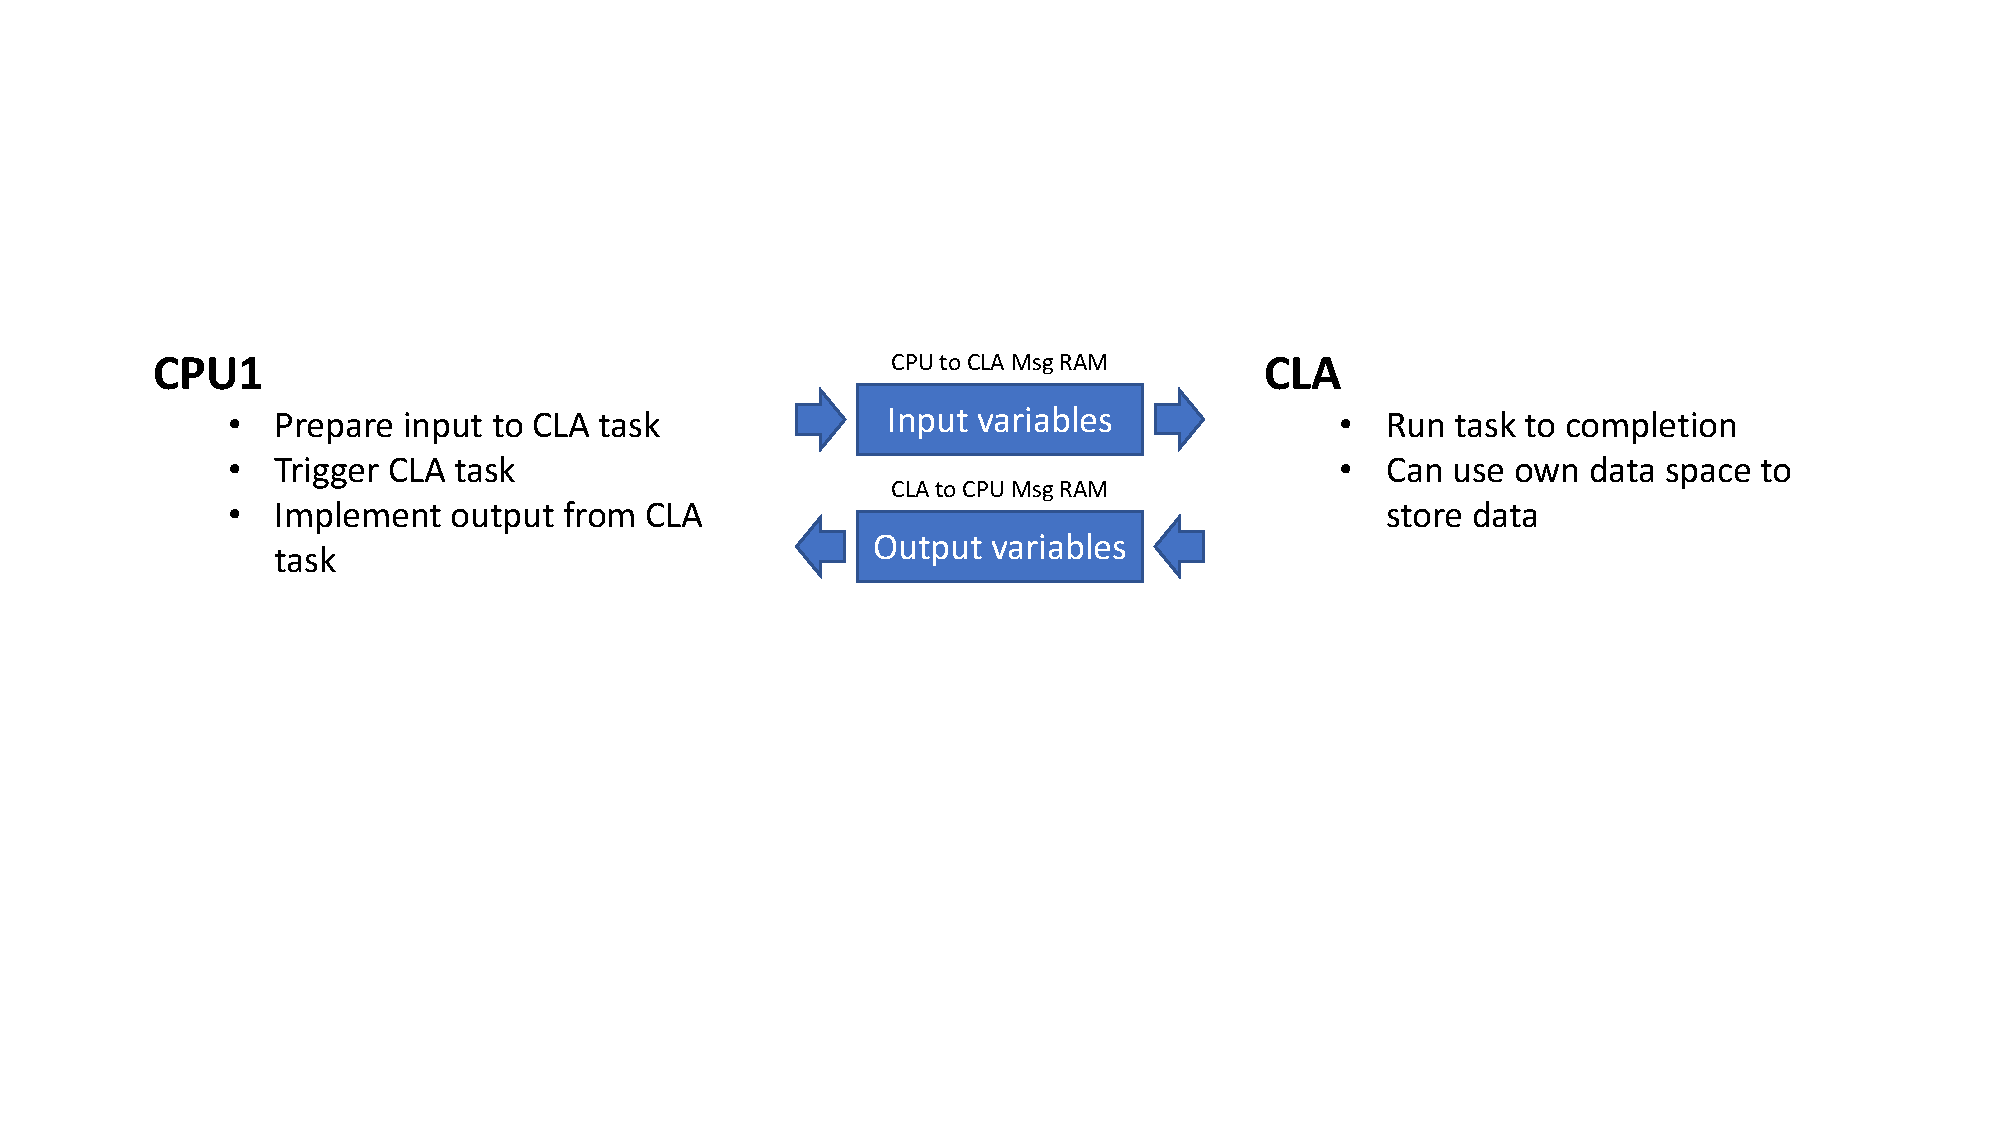
\includegraphics[width=1.0\textwidth]{./figures/CLA_communication.pdf}
    \caption{Communication of inputs and outputs for CLA tasks.}
    \label{fig:CLA_communication}
\end{figure}

\section{Debugging}

During development it can be useful to print messages to a console. For this purpose I configured a third SCI interface on the micro-controller that is connected to a USB-to-Serial converter on the XDS100v2 On-Board Debug Probe of the Launchpad. Using this serial interface the micro-controller can print messages to a host computer. However, in order to make use of support functions such as \mintinline{c}{printf()} the default Runtime Support Library requires a lot of code and the use of a heap. To avoid these heavy functions I instead used the tinyprintf library\cite{tinyprintf} which is specifically designed for embedded systems and implements all standard functions such as \mintinline{c}{printf()}.

Printing messages to the console is synchronous and blocking. However, this is acceptable since  printing is not intended for production and is removed in the final build.

While CPU1 can easily output messages over serial, as it is the master of the SCI peripheral, the same is not true for CPU2. Instead of switching the master of the SCI, which would be prone to glitches, CPU2 uses IPC message registers to pass characters to CPU1. An IPC flag is then configured to cause an interrupt on CPU1. The interrupt service routine then prints the character received from CPU2. This mechanism provides both core with the ability to print debug messages to a console. However, it is important to keep in mind, that this mechanism does not provide and form of locking.

\section{Unit Testing}

In order to ensure correctness, extensive unit tests are employed to test all critical control algorithms and any other modules that can reasonably be tested using software tests. The implemented unit tests specifically also test limits and edge cases that could lead to numerical errors such as integer overflows and underflows. If enabled at compile-time, unit tests execute just before the main loop is entered. However, unit tests are not intended to execute in production, as they may lead to an undesired state and reconfigure some parts of the system for testing.
